\documentclass[11pt,a4paper]{beamer}
\usepackage[utf8]{inputenc}
%\usepackage[english]{babel}
\usepackage[T1]{fontenc}
\usepackage{amsmath}
\usepackage{amsthm}
\usepackage{amssymb}
\usepackage{amstext}

\usetheme		{Warsaw}%,Malmoe,Warsaw,3kolonky:CambridgeUS,Madrid %%Ilmenau,Antibes,,,,Luebeck,Copenhagen,
%\beamertemplateballitem
\usecolortheme	{orchid}%crane, orchid

\author{Bc. Jan Kučera}
\title{Rényi pseudo-distances}
\institute{FNSPE, CTU \\ $\quad$  \\ Work supervisor: Ing. Václav Kůs Ph.D.}
\date{26.6.2012}

\newcommand{\intpa}{\int p_\theta^{1+\alpha}(x) \, \mathrm{d}x }
\newcommand{\fn}{\frac{1}{n} \sum_{i=1}^n p_{\theta}^{\alpha}\left( x_i \right)}
\newcommand{\fln}{\frac{1}{n} \sum_{i=1}^n \ln p_{\theta}\left( x_i \right)}
\newcommand{\Cat}{C_\alpha\left( \theta \right)}
\newcommand{\amtiT}{\arg \max_{\theta \in \Theta}}
\newcommand{\fa}{\frac{\alpha}{1+\alpha}}


\begin{document}

\begin{frame}
	\maketitle
\end{frame}

\begin{frame}{Table of contents}
    	\tableofcontents
\end{frame}

%
%\begin{frame}
%	Let $\mathcal{P} = \lbrace P_\theta : \theta \in \Theta \subset \mathbb{R}^m \rbrace$ be set of probability measures on $\left(\mathcal{X},\mathcal{A}\right)$. \\
%	Let $Q$ probability measure on $\left(\mathcal{X},\mathcal{A}\right)$. \\
%	Let $X_1,\ldots,X_n$ be i.i.d observations governed by convex mixtures $\tilde{P} = (1-\epsilon) P_\theta + \epsilon Q$. We denote $\mathcal{\tilde{P}} = \mathcal{P} \cup \lbrace \tilde{P} \rbrace$
%\end{frame}

\section{Decomposable pseudo-distance} %******************************************** PSEUDO-DISTANCE
\begin{frame}{Decomposable pseudo-distance}
		We say, that $\mathfrak{D}:\mathcal{P} \rightarrow \mathbb{R}$ is \emph{pseudo-distance} if $\forall P,Q\in\mathcal{P}$
		\begin{equation*}
			\mathfrak{D}(P,Q) \geq 0  \qquad \text{and} \qquad \mathfrak{D}(P,Q)=0 \; \Leftrightarrow \; P=Q
		\end{equation*}
		 and this pseudo-distance is \emph{ decomposable} if there exist functionals so that
		 $\mathfrak{D}^0:\mathcal{P}\rightarrow\mathbb{R}$, $ \mathfrak{D}^1:\mathcal{\tilde{P}} \rightarrow \mathbb{R}$ and measurable  
		  $\rho_\theta : \mathcal{X} \rightarrow \mathbb{R}$, $ \theta \in \Theta$, so that $\forall \theta \in \Theta$ and $\forall Q \in \mathcal{\tilde{P}}$ there exists finite $\int{\rho_\theta }\mathrm{d}Q$ and
		\begin{equation*}
			\mathfrak{D} (P_\theta, Q) = \mathfrak{D}^0 (P_\theta) + \mathfrak{D}^1 (Q) + \int \rho_\theta \mathrm{d}Q.
		\end{equation*}
		\begin{itemize}
			\item we don't presume triangle inequality or symmetry
		\end{itemize}			
\end{frame}

%\begin{frame}
%	\begin{itemize}
%		\item methods based on minimization of some functional
%		
%	\end{itemize}
%\end{frame}

\begin{frame}{Minimal distance estimator}
	Functional $T_\mathfrak{D}:\mathcal{\tilde{P}} \rightarrow \Theta$ defines \emph{minimal distance} estimator if $\mathfrak{D}(P_\theta,Q)$ is decomposable and $T_\mathfrak{D}(Q) \in \Theta$ minimizes 
	\begin{equation*}
		T_\mathfrak{D}(Q) = \arg \min_{\theta \in \Theta} \left[ \mathfrak{D}^0 (P_\theta) + \int \rho_\theta \mathrm{d}Q \right], \quad \forall Q \in \mathcal{\tilde{P}}
	\end{equation*}
\end{frame}

\section{Rényi pseudo-distance} % ************************************************ RENYI PSEUDO-DISTANCE

\begin{frame}{Rényi pseudo-distance}
	Let for some $\beta>0$
	\begin{equation*}
			p^\beta, q^\beta,\ln{p} \in \mathrm{L}_1(Q), \quad \forall P \in \mathcal{P}, Q \in \mathcal{\tilde{P}}.
	\end{equation*}
	holds. Then for some $\alpha$, $0 < \alpha \leq \beta,\; P \in \mathcal{P}, \; Q \in \mathcal{\tilde{P}} $ is decomposable, that is 
	\begin{equation*}
		\mathcal{R}_\alpha (P,Q) = \mathcal{R}_\alpha^0 (P) + \mathcal{R}_\alpha^1 (Q) - \dfrac{1}{\alpha} \ln{\left( \int{p^\alpha \mathrm{d}Q } \right)},
	\end{equation*}	
	where 
	\begin{equation*}
		\mathcal{R}_\alpha^0 (P) = \dfrac{1}{1+\alpha}\ln{\left( \int{p^\alpha \mathrm{d}P } \right)}, \quad \mathcal{R}_\alpha^1 (Q) = \dfrac{1}{\alpha (1+\alpha)}\ln{\left( \int{q^\alpha \mathrm{d}Q } \right)}.
	\end{equation*}
	Moreover for $\alpha \searrow 0$
	\begin{equation*}
		\mathcal{R}_0 (P,Q) = \int{\left( \ln{q} - \ln{p} \right)\mathrm{d}Q}
	\end{equation*}
\end{frame}

%\begin{frame}
%	Rényi distance estimator is then
%	\begin{equation*}
%		T_{\mathfrak{R}_\alpha} = 
%		\begin{cases}
%				\arg\min_\theta \left[ \dfrac{1}{1+\alpha}\ln{\left( \int{p_\theta^\alpha \mathrm{d}P_\theta} \right)} - \dfrac{1}{\alpha}\ln{\left( \int{p^\alpha_\theta \mathrm{d}Q } \right)} \right], \\
%				\qquad \text{for } \, 0<\alpha \leq \beta \\
%				\arg\min_\theta  - \ln{\left( \int{p_\theta \mathrm{d}Q}  \right)}, \\
%				\qquad \text{for } \,  \alpha = 0.
%		\end{cases}
%	\end{equation*}
%\end{frame}

\begin{frame}
If we replace Q by the empirical distribution $P_n$, we get
\begin{equation*}
	\theta_{\mathfrak{R}_\alpha,n} = 
	\begin{cases}
		\displaystyle{ \amtiT \left( \intpa \right)^{-\frac{\alpha}{1+\alpha}} \fn }, \\
		\qquad \text{for } 0 < \alpha \leq \beta, \\
		\displaystyle{ \amtiT  \fln },\\
		\qquad \text{for } \alpha = 0.
	\end{cases}	
\end{equation*}
	So for $\alpha = 0 $ the $\theta_{\alpha,n} = \theta_{MLE}$
\end{frame}

\section{Applications for distributions}
\subsection{Normal distribution}   %%%%%%%%%%%%%%    NORMAL    ********************************************************************************
\begin{frame}{Normal distribution}
	\begin{equation*}
		p_\theta = \frac{1}{\sqrt{2\pi\sigma^2}}\exp{\left[ -\frac{(x-\mu)^2}{2\sigma} \right]}
	\end{equation*}
	\begin{equation*}
		\theta_{\mathfrak{R}_\alpha,n} = \amtiT \frac{1}{n\sigma^{\frac{\alpha}{1+\alpha}}} \sum_{i=1}^n \exp \left[ -\alpha \frac{(x_i - \mu)^2}{2\sigma^2} \right]		
	\end{equation*}
\end{frame}

\begin{frame}
	distances in the parametric space:
	\begin{center}
		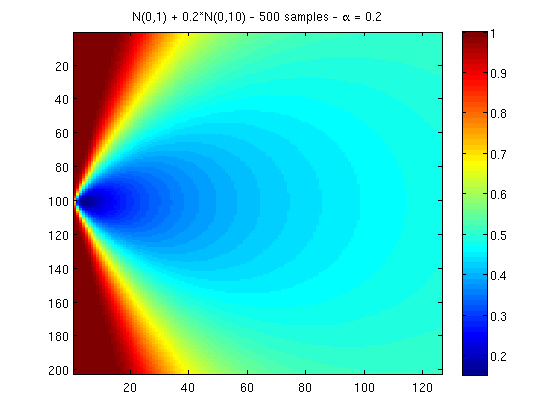
\includegraphics[width = 3in]{vzdalenosti-02-500-02.png}			
	\end{center}
\end{frame}

\begin{frame}
	\begin{equation*}
		\mathrm{IF}(x;T_{\mathfrak{R}_\alpha},\mu) = (1+\alpha )^{\frac{3}{2}} (x-\mu ) e^{-\frac{\alpha}{2} (x-\mu )^2} 
	\end{equation*}
	\begin{center}
		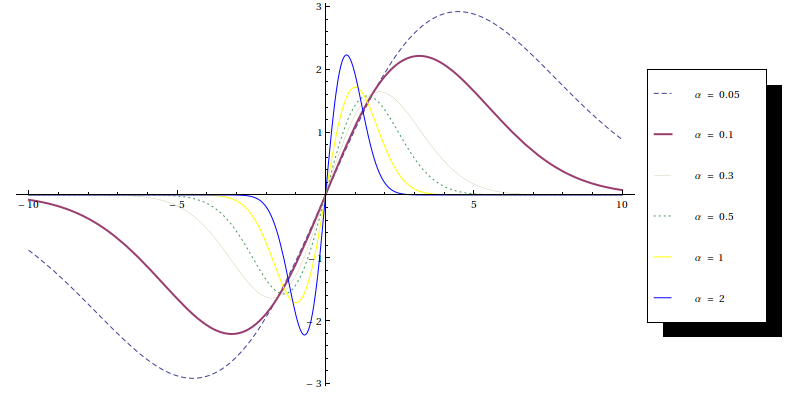
\includegraphics[width = 4in]{IF-Normal-mu.png}			
	\end{center}
\end{frame}


\begin{frame}
	\begin{equation*}
		\mathrm{IF}(x;T_{\mathfrak{R}_\alpha},\sigma) = \frac{(1+\alpha)^\frac{5}{2}\sigma}{2} \left(\left(\frac{x}{\sigma} \right)^2 - \frac{1}{1+\alpha} \right) e^{ -\frac{\alpha x^2}{2\sigma^2}}
	\end{equation*}
	\begin{center}
		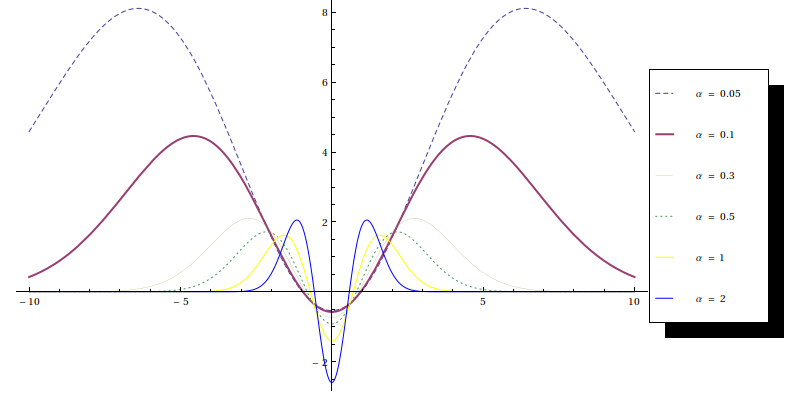
\includegraphics[width = 4in]{IF-Normal-sigma.png}			
	\end{center}
\end{frame}

\begin{frame}
	$\lim_{x\rightarrow \pm\infty}\mathrm{IF}(x;T_{\mathfrak{R}_\alpha},\cdot) = 0 $ \\
	$\rightarrow$ estimator is robust against outliers \\
	$\sup_{x}{|\mathrm{IF}(x;T_{\mathfrak{R}_\alpha},\cdot)|}$   is finite \\
		$\rightarrow$ estimator is robust against point errors

\end{frame}

\begin{frame} 
\begin{table}[ht] \footnotesize 
\begin{center} 
\begin{tabular}{|c|ccc|} 
\hline 
$\alpha\backslash n$ &&  $500$ & \\ 
\hline 
& $m(\mu)$ & $s(\mu)$ & $eref(\mu)$  \\ 
& $m(\sigma)$ & $s(\sigma)$ & $eref(\sigma)$ \\ 
\hline 
$0.0$ & $ 0.000 $ & $ 0.037 $ & $ 1.000 $\\ 
 & $ 1.672 $ & $ 0.051 $ & $ 1.000 $\\ 
\hline 
$0.01$ &  $ -0.000 $ & $ 0.037 $ & $ 1.032 $\\ 
 & $ 1.652 $ & $ 0.050 $ & $ 1.031 $\\ 
\hline 
$0.05$ &  $ 0.001 $ & $ 0.033 $ & $ 1.248 $\\ 
 &$ 1.572 $ & $ 0.046 $ & $ 1.244 $\\ 
\hline 
$0.1$ & $ -0.000 $ & $ 0.031 $ & $ 1.426 $\\ 
 &  $ 1.478 $ & $ 0.041 $ & $ 1.560 $\\ 
\hline 
$0.2$ & $ -0.000 $ & $ 0.029 $ & $ 1.650 $\\ 
 & $ 1.333 $ & $ 0.035 $ & $ 2.097 $\\ 
\hline 
$0.5$ & $ -0.000 $ & $ 0.028 $ & $ 1.733 $\\ 
 &  $ 1.156 $ & $ 0.028 $ & $ 3.295 $\\ 
\hline 
\end{tabular}
\caption{Renyi: $p = \mathrm{N}(0,1)$, data: $(1-\varepsilon)\mathrm{N}(0,1) + \varepsilon \mathrm{N}(0,10)$, $\varepsilon =  0.2$, $K = 10000$} 
\end{center}
\end{table}
\end{frame}

\begin{frame}
	\begin{table}[ht] \footnotesize 
\begin{center} 
\begin{tabular}{|c|ccc|} 
\hline 
$\alpha\backslash n$ &&  $500$ & \\ 
\hline 
& $m(\mu)$ & $s(\mu)$ & $eref(\mu)$ \\ 
& $m(\sigma)$ & $s(\sigma)$ & $eref(\sigma)$\\ 
\hline 
$0.0$ & $ -0.000 $ & $ 0.021 $ & $ 1.000 $\\ 
 & $ 0.949 $ & $ 0.016 $ & $ 1.000 $\\ 
\hline 
$0.01$ &  $ -0.000 $ & $ 0.021 $ & $ 1.002 $\\ 
 &  $ 0.949 $ & $ 0.016 $ & $ 0.969 $\\ 
\hline 
$0.05$ & $ 0.001 $ & $ 0.021 $ & $ 0.991 $\\ 
 &  $ 0.945 $ & $ 0.016 $ & $ 0.967 $\\ 
\hline 
$0.1$ & $ 0.000 $ & $ 0.021 $ & $ 0.990 $\\ 
 & $ 0.942 $ & $ 0.017 $ & $ 0.889 $\\ 
\hline 
$0.2$ &  $ -0.001 $ & $ 0.021 $ & $ 1.032 $\\ 
 & $ 0.931 $ & $ 0.017 $ & $ 0.865 $\\ 
\hline 
$0.5$ &  $ -0.000 $ & $ 0.021 $ & $ 0.998 $\\ 
 & $ 0.905 $ & $ 0.020 $ & $ 0.641 $\\ 
\hline 
\end{tabular}
\caption{Renyi: $p = \mathrm{N}(0,1)$, data: $0.9\mathrm{N}(0,1) + 0.1\mathrm{N}_{0.1x}(0,1)$, $K = 1000$} 
\end{center}
\end{table}
\end{frame}

\begin{frame}
\begin{table}[ht] \footnotesize 
\begin{center} 
\begin{tabular}{|c|ccc|} 
\hline 
$\alpha\backslash n$ &&  $500$ & \\ 
\hline 
& $m(\mu)$ & $s(\mu)$ & $eref(\mu)$ \\ 
& $m(\sigma)$ & $s(\sigma)$ & $eref(\sigma)$ \\ 
\hline 
$0.0$ & $ -0.002 $ & $ 0.075 $ & $ 1.000 $\\ 
 &  $ 3.294 $ & $ 0.231 $ & $ 1.000 $\\ 
\hline 
$0.01$& $ -0.000 $ & $ 0.065 $ & $ 1.327 $\\ 
 & $ 3.104 $ & $ 0.220 $ & $ 1.103 $\\ 
\hline 
$0.05$ & $ 0.001 $ & $ 0.040 $ & $ 3.489 $\\ 
 &  $ 2.118 $ & $ 0.189 $ & $ 1.493 $\\ 
\hline 
$0.1$ &  $ 0.001 $ & $ 0.026 $ & $ 8.356 $\\ 
 & $ 1.277 $ & $ 0.053 $ & $ 18.986 $\\ 
\hline 
$0.2$ &  $ 0.000 $ & $ 0.025 $ & $ 8.796 $\\ 
 & $ 1.087 $ & $ 0.024 $ & $ 91.365 $\\ 
\hline 
$0.5$ &$ -0.000 $ & $ 0.026 $ & $ 8.390 $\\ 
 & $ 1.029 $ & $ 0.021 $ & $ 123.291 $\\ 
\hline 
\end{tabular}
\caption{Renyi: $p = \mathrm{N}(0,1)$, data: $0.9\mathrm{N}(0,1) + 0.1\mathrm{N}_{10.0x}(0,1)$, $K = 1000$} 
\end{center}
\end{table}
\end{frame}

%\subsection{Cauchy distribution}    %%%%%%%%%%%%%%    CAUCHY    ********************************************************************************
%\begin{frame}{Cauchy distribution}
%	\begin{equation*}
%		p_\theta = \frac{1}{\pi\sigma} \left( 1 + \left( \frac{x-\mu}{\sigma} \right)^2 \right)^{-1}
%	\end{equation*}
%	\begin{equation*}
%		\theta_{\mathfrak{R}_\alpha,n} = \amtiT \sigma^{-\frac{\alpha}{1+\alpha}} \frac{1}{n} \sum_{i=1}^n \left( 1 + \left( \frac{x_i-\mu}{\sigma} \right)^2 \right)^{-\alpha} \nonumber
%	\end{equation*}
%	\begin{equation*}
%		\mathrm{IF}(x;T_{\mathfrak{R}_\alpha},\mu) = \sqrt{\pi}\frac{\Gamma\left( 3 + \alpha \right)}{\Gamma\left( \frac{3}{2} + \alpha \right)} \left( \frac{1}{1 + (x-\mu)^2}\right)^{1+\alpha}(x-\mu) 
%	\end{equation*}
%\end{frame}

\subsection{Laplace distribution}    %%%%%%%%%%%%%%    LAPLACE    ********************************************************************************
\begin{frame}{Laplace distribution}
	\begin{equation*}
		p_\theta = \frac{1}{2\lambda} e^{-\frac{|x-\mu|}{\lambda}}
	\end{equation*}
	\begin{equation*}
		\theta_{\mathfrak{R}_\alpha,n} = \amtiT (2\lambda)^{-\frac{\alpha}{1+\alpha}} \frac{1}{n} \sum_{i=1}^n \exp \left[-\alpha\frac{|x_i-\mu|}{\lambda} \right]
	\end{equation*}
\end{frame}

\begin{frame}
	\begin{equation*}
		\mathrm{IF}(x;T_{\mathfrak{R}_\alpha},\mu) = (1+\alpha )^{\frac{3}{2}} (x-\mu )  e^{-\frac{\alpha}{2} (x-\mu )^2}% IF(x,mu)
	\end{equation*}

	\begin{center}
		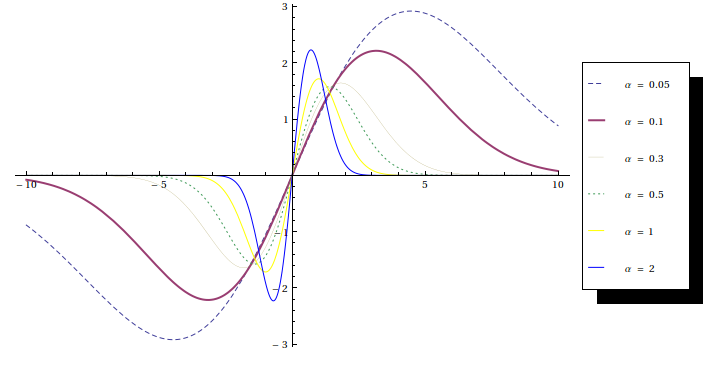
\includegraphics[width = 3.1in]{IF-Laplace-mu.png}			
	\end{center}
\end{frame}

\begin{frame}
	\begin{equation*}
		\mathrm{IF}(x;T_{\mathfrak{R}_\alpha},\lambda) = (1 + \alpha)^2 \left(-\lambda + (1 + \alpha)|x|\right)  e^{-\frac{\alpha|x|}{\lambda}}	 % IF(x,sigma)
	\end{equation*}
	\begin{center}
		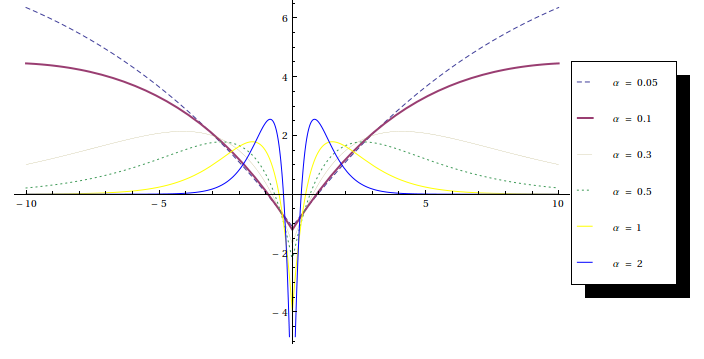
\includegraphics[width = 3.1in]{IF-Laplace-sigma.png}			
	\end{center}
\end{frame}

\begin{frame}
\begin{table}[ht] \tiny 
\begin{center} 
\begin{tabular}{|c|ccc|} 
\hline 
$\alpha\backslash n$ &&  $500$ & \\ 
\hline 
& $m(\mu)$ & $s(\mu)$ & $eref(\mu)$ \\ 
& $m(\lambda)$ & $s(\lambda)$ & $eref(\lambda)$ \\ 
\hline 
$0.0$ & $ 0.000 $ & $ 0.065 $ & $ 1.000 $\\ 
 & $ 3.723 $ & $ 0.355 $ & $ 1.000 $\\ 
\hline 
$0.01$ & $ 0.003 $ & $ 0.063 $ & $ 1.090 $\\ 
 & $ 3.593 $ & $ 0.338 $ & $ 1.102 $\\ 
\hline 
$0.05$ &  $ 0.002 $ & $ 0.063 $ & $ 1.063 $\\ 
 &  $ 3.239 $ & $ 0.306 $ & $ 1.348 $\\ 
\hline 
$0.1$ &  $ -0.002 $ & $ 0.062 $ & $ 1.118 $\\ 
 &  $ 2.796 $ & $ 0.285 $ & $ 1.556 $\\ 
\hline 
$0.2$  & $ 0.000 $ & $ 0.062 $ & $ 1.105 $\\ 
 & $ 2.059 $ & $ 0.205 $ & $ 3.005 $\\ 
\hline 
$0.3$ & $ -0.003 $ & $ 0.060 $ & $ 1.198 $\\ 
 &  $ 1.626 $ & $ 0.154 $ & $ 5.326 $\\ 
\hline 
$0.5$ &  $ 0.000 $ & $ 0.058 $ & $ 1.267 $\\ 
 &  $ 1.300 $ & $ 0.108 $ & $ 10.756 $\\ 
\hline 
$1.0$ &  $ -0.001 $ & $ 0.068 $ & $ 0.932 $\\ 
 &  $ 1.126 $ & $ 0.110 $ & $ 10.386 $\\ 
\hline 
\end{tabular}
\caption{Renyi: $p = \mathrm{L}(0,1)$, data: $(1-\varepsilon)\mathrm{L}(0,1) + \varepsilon \mathrm{L}(0,10)$, $\varepsilon =  0.3$, $K = 1000$} 
\end{center}
\end{table}
\end{frame}



\subsection{Exponential distribution}
\begin{frame}{Exponential distribution} %%%%%%%%%%%%%%%    EXPONENTIAL    *************************************************************************
	\begin{equation*}
		p_\theta = \frac{1}{\lambda} e^{-\frac{x-\mu}{\lambda}  }
	\end{equation*}
	\begin{equation*}
		\theta_{\mathfrak{R}_\alpha,n} = \amtiT \lambda^{-\frac{\alpha}{1+\alpha}} \frac{1}{n}\sum_{i=1}^n \exp \left[-\alpha\frac{x_i-\mu}{\lambda} \right]
	\end{equation*}
	
	
\end{frame}

\begin{frame}
	\begin{equation*}
		\mathrm{IF}(x;T_{\mathfrak{R}_\alpha},\mu) = e^{-\frac{\alpha}{2} (x-\mu )^2} (1+\alpha )^{\frac{3}{2}} (x-\mu )
	\end{equation*}
	\begin{center}
		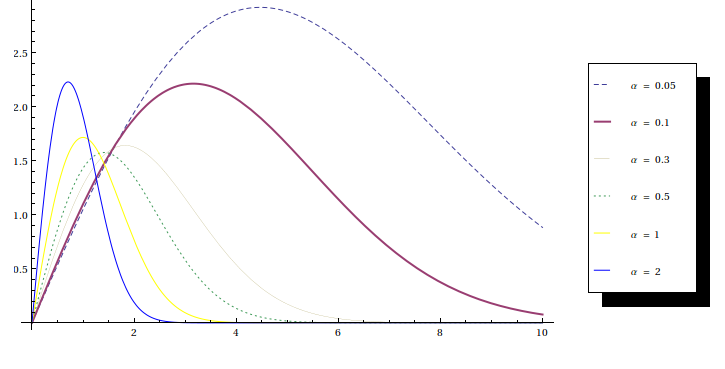
\includegraphics[width = 3.1in]{IF-Exponential-mu.png}			
	\end{center}
\end{frame}

\begin{frame}
	\begin{equation*}
		\mathrm{IF}(x;T_{\mathfrak{R}_\alpha},\lambda) =	(1+\alpha )^2 ( - \lambda +(1+ \alpha)x) e^{-\frac{\alpha x}{\lambda }}
	\end{equation*}
	\begin{center}
		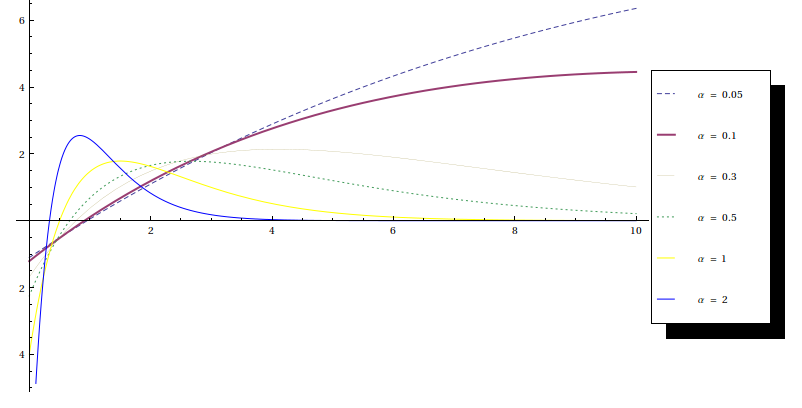
\includegraphics[width = 3.1in]{IF-Exponential-sigma.png}			
	\end{center}
\end{frame}

\begin{frame}
\begin{table}[ht] \footnotesize
\begin{center} 
\begin{tabular}{|c|ccc|} 
\hline 
$\alpha\backslash n$ && $500$ & \\ 
\hline 
& $m(\lambda)$ & $s(\lambda)$ & $eref(\lambda)$ \\ 
\hline 
$0.0$ & $ 3.901 $ & $ 0.432 $ & $ 1.000 $\\ 
\hline 
$0.01$ &$ 3.614 $ & $ 0.356 $ & $ 1.475 $\\ 
\hline 
$0.05$ & $ 3.241 $ & $ 0.317 $ & $ 1.862 $\\ 
\hline 
$0.1$ & $ 2.796 $ & $ 0.274 $ & $ 2.495 $\\ 
\hline 
$0.15$ & $ 2.389 $ & $ 0.239 $ & $ 3.258 $\\ 
\hline 
$0.2$ &$ 2.049 $ & $ 0.209 $ & $ 4.281 $\\ 
\hline 
$0.3$ & $ 1.622 $ & $ 0.153 $ & $ 7.999 $\\ 
\hline 
$0.5$ &  $ 1.310 $ & $ 0.110 $ & $ 15.330 $\\ 
\hline 
$1.0$ &  $ 1.139 $ & $ 0.109 $ & $ 15.806 $\\ 
\hline 
\end{tabular}
\caption{Renyi: $p = \mathrm{E}(0,1)$, data: $(1-\varepsilon)\mathrm{E}(0,1) + \varepsilon \mathrm{E}(0,10)$, $\varepsilon =  0.3$, $K = 1000$} 
\end{center}
\end{table}
\end{frame}

\subsection{Weibull distribution}
\begin{frame}{Weibull distribution} %%%%%%%%%%%%%%     WEIBULL     *******************************************************
	\begin{equation*}
		p_\theta =  \frac{k}{\lambda} \left( \frac{x-\mu}{\lambda} \right)^{k-1} \exp \left[ -\left( \frac{x-\mu}{\lambda} \right)^k \right] 
	\end{equation*}
	\begin{eqnarray}
		\theta_{\mathfrak{R}_\alpha,n} & = & \amtiT \left( \frac{k}{\lambda} \right)^\fa (1+\alpha)^{\fa\frac{1+\alpha+k}{k}} \Gamma\left(\frac{1+\alpha+k}{k}\right)^{-\fa} \nonumber \\
							&& \frac{1}{n}\sum_{i=1}^n \left( \frac{x_i-\mu}{\lambda}\right)^{\alpha(k-1)} \exp\left[-\alpha \left(\frac{x_i-\mu}{\lambda}\right)^k\right] \nonumber
	\end{eqnarray}
\end{frame}

\begin{frame}
\begin{table}[ht] \footnotesize 
\begin{center} 
\begin{tabular}{|c|ccc|} 
\hline 
$\alpha\backslash n$ &&  $500$ & \\ 
\hline 
& $m(\lambda)$ & $s(\lambda)$ & $eref(\lambda)$ \\ 
\hline 
$0.0$ & $ 4.713 $ & $ 0.387 $ & $ 1.000 $\\ 
\hline 
$0.01$ & $ 4.568 $ & $ 0.364 $ & $ 1.130 $\\ 
\hline 
$0.05$ & $ 4.149 $ & $ 0.373 $ & $ 1.077 $\\ 
\hline 
$0.1$ &$ 3.511 $ & $ 0.383 $ & $ 1.020 $\\ 
\hline 
$0.15$ & $ 2.574 $ & $ 0.428 $ & $ 0.815 $\\ 
\hline 
$0.2$ & $ 1.664 $ & $ 0.261 $ & $ 2.201 $\\ 
\hline 
$0.3$ &  $ 1.226 $ & $ 0.076 $ & $ 25.766 $\\ 
\hline 
$0.5$ & $ 1.096 $ & $ 0.057 $ & $ 46.725 $\\ 
\hline 
$1.0$ & $ 1.043 $ & $ 0.055 $ & $ 49.962 $\\ 
\hline 
\end{tabular}
\caption{Renyi: $p = \mathrm{W}(1.5,1)$, data: $(1-\varepsilon)\mathrm{W}(1.5,1) + \varepsilon \mathrm{W}(1.5,10)$, $\varepsilon =  0.3$, $K = 1000$} 
\end{center}
\end{table}
\end{frame}
%
%\section{}
%\begin{frame}{Conclusion}
%	Rényi pseudo-distance
%	\begin{itemize}
%		\item can filter out outliers when distribution is poluted with another distribution with heavier tail
%		
%	\end{itemize}
%\end{frame}

\begin{frame}
	\begin{center}
		Thank you for your attention.
	\end{center}
\end{frame}

\end{document}


























